% ===========================================
% Digital Logic
% Written by: Braidan Duffy
%
% Date: 07/06/2022
% Last Revision: 07/06/2022
% ============================================

\setchapterstyle{kao}
\chapter{Digital Electronics}
\setchapterpreamble[u]{\margintoc}
\labch{digital_electronics}

Computers have existed in some fashion or another for millennia.
The ancient antikythera mechanism was a hand-powered computer that predicted the position of astronomical bodies throughout the year.
Mathematicians in the 18th and 19th centuries used complicated machines and mechanisms to run calculus and trigonometric calculations at speeds way faster than possible by humans by hand.
Then, in the mid-1940's nations used analog computers to compute the trajectories of ballistic projectiles and free falling bombs.
Today, analog computers are still used in niche applications, but since the transistor revolution of the 1960's and 1970's, almost every computer in the world has transitioned to digital logic.

\section[Introduction to Binary]{Introduction to Binary}
Digital logic is electrically simple to implement: either current flows (a logical '1') or it does not (a logical '0').
Even better, the circuit required to calculate digital logic can be generalized or reconfigured, depending on the architecture used.
This makes digital logic a far more versatile tool compared to analog computers which can only be made for specific applications.

The fundamentals of computing are above the scope of these notes, but it is still important for engineers to understand the basic logic behind digital computations and know about the 1's and 0's that dictate our modern lifestyles

\paragraph*{What is Binary?} Binary is the representation of the state of an object.
As the latin prefix implies, there are two states represented by binary: on (logical '1') or off (logical '0').
A lightbulb is a good example of a binary object - it is either on, lighting up a room, or off, leaving the room in darkness.

Binary is fundamentally a numbering system, much like the arabic numerals we use in our day-to-day lives.
Arabic numerals are in Base10, meaning we comprehend counting in multiples of 10 using the digits 0-9. For example:
\begin{align*}
    20     &= 10*2 \\
    450    &= 4*10*10 + 5*10 \\
    245683 &= 2*10^5 + 4*10^4 + 5*10^3 + 6*10^2 + 8*10^1 + 3*10^0
\end{align*}

Binary is counted in Base2, meaning everything is counted in multiples of 2 using the digits 0 and 1. Using the same example as before:
\begin{align*}
    20     &= 2^5 + 2^3 \\
    450    &= 2^8 + 2^7 + 2^6 + 0^5 + 0^4 + 0^3 + 0^2 + 2^1 + 0^0 \\
    245683 &= 2^{17} + 2^{16} + 2^{15} + 2^{13} + 2^{12} + 2^{11} + 2^{10} + 2^9 + 2^8 + 2^7 + 2^5 + 2^4 + 2^1 + 2^0
\end{align*}
        
While this is inefficient for a human to understand its meaning, a computer can quickly transform this on/off pattern of electrons into numbers for calculations.

Binary numbers are broken down into three groupings: bits (one number), nibbles (four bits), and bytes (two nibbles or eight bits). 
The groupings are extremely important as the order and number of the bits in a binary representation dictate the number or logical input used in the calculation.
Each bit is indexed starting from 0, as shown in \hl{FIGURE} and goes from the Least Significant Bit (LSB) at index 0, to the Most Significant Bit (MSB) at the furthest index. 
\sidenote{These indecies get their names because of how they affect the binary number when changed. 
The LSB only changes the numerical value by 1.
The MSB, on the other hand, can change the value by upto an infinite value, depending on how many bits are present in the binary number}

\begin{figure*}
    \labfig{byte_breakdown}
    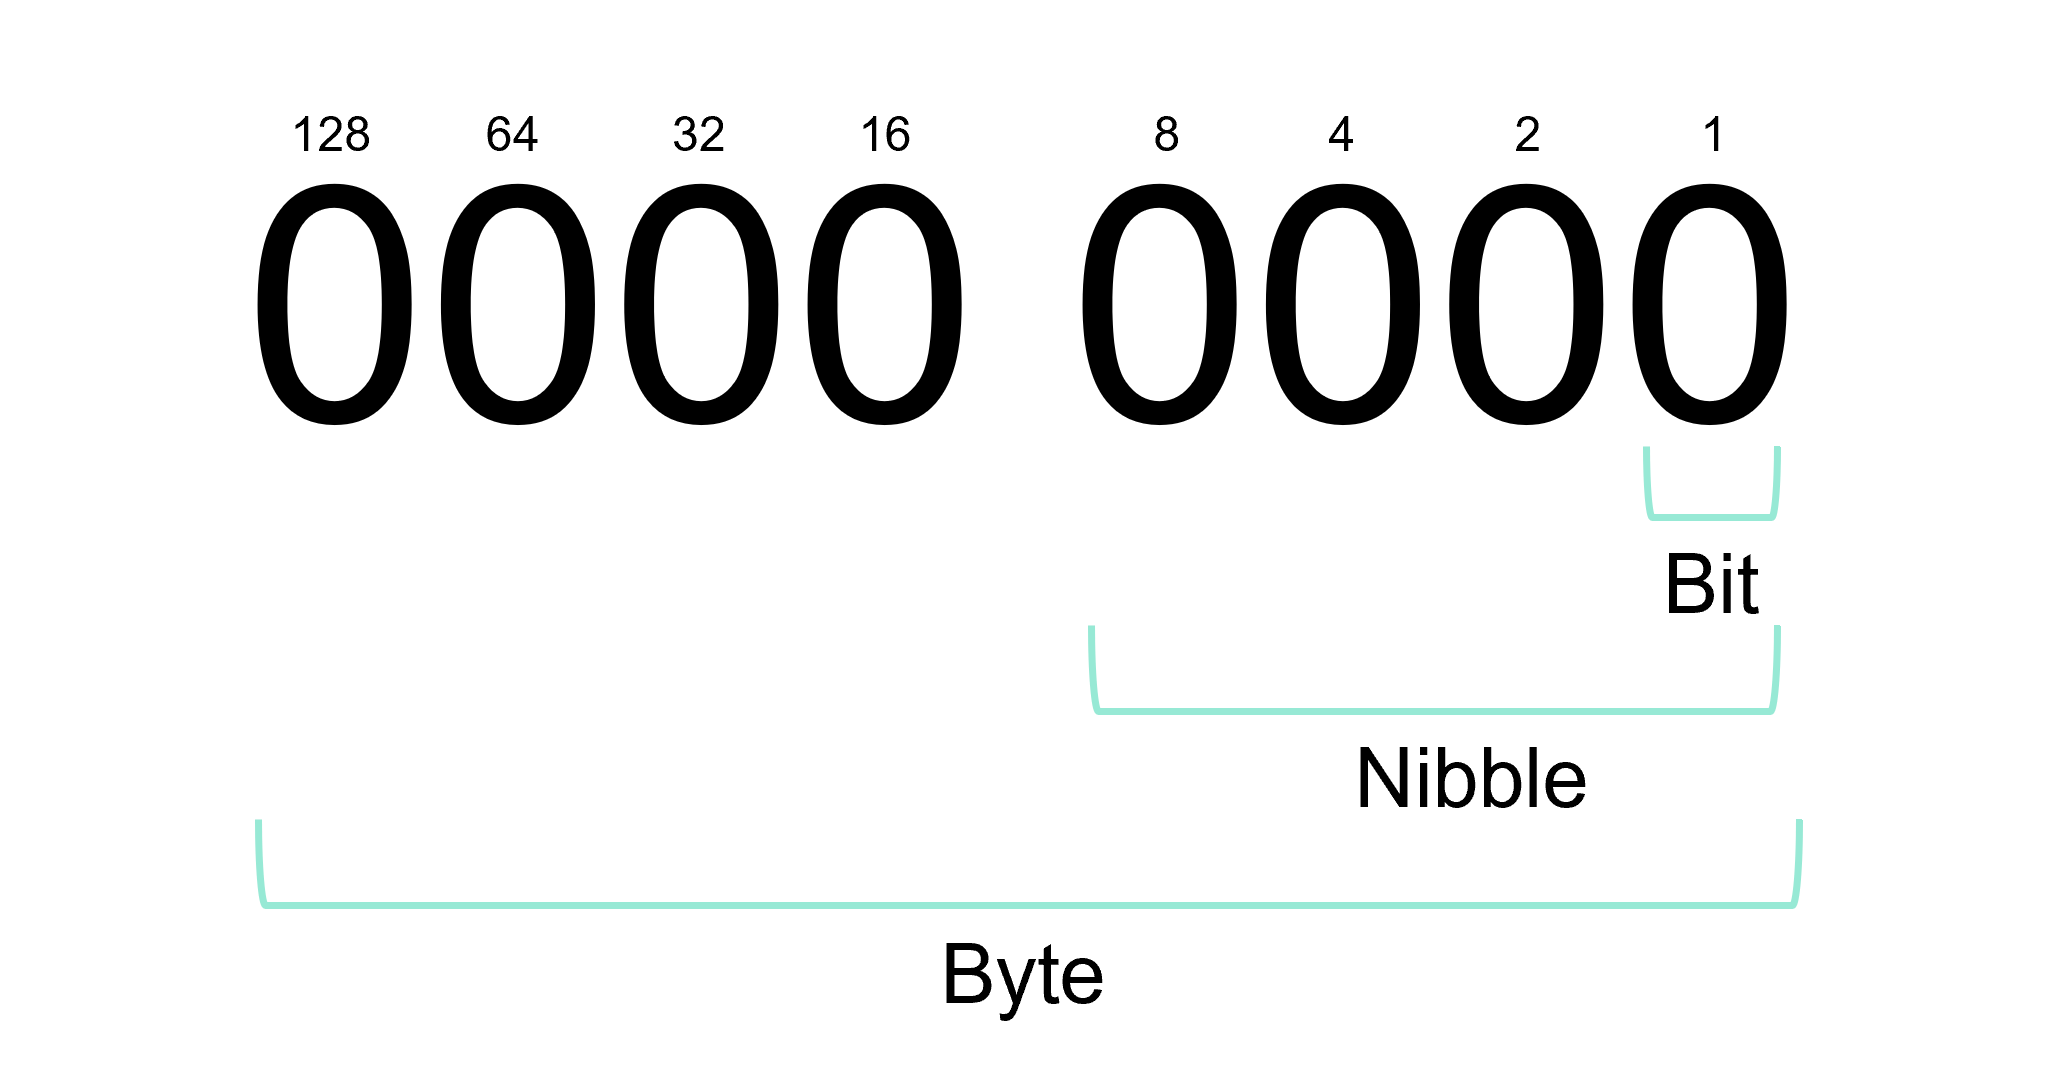
\includegraphics[height=2.5in]{digital_logic/bit-breakdown.png}
    \caption[Byte Breakdown]{Breakdown of a byte from the largest unit, to the smallest, with indexing.}
\end{figure*}

    \subsection{Binary Arithmetic}
    Much like our beloved arabic numerals, binary numbers can be added, subtracted, multiplied, and divided.

    \paragraph*{Addition} Adding binary numbers is straight-forward.
    Simply stack the numbers you wish to add on top of each other, ensuring the indices align.
    Note, binary addition is commutative, meaning the number order does not matter, so long as the indices are aligned.
    Then, for each index, add the numbers together.
    If the result is greater than 1, then set the result of the index addition to 0 and carry a '1' over to the next index.
    Repeat until you have calculated the last index!

    \begin{example}[Adding binary numbers]
        Let's add $7_{10}$ ($0111_2$) and $11_{10}$ ($1011_2$):
        \begin{center}
            \begin{tabular}{ccccc}
                $^1$  & $0^1$ & $1^1$ & $1^1$ & $1$ \\
                +     & 1     & 0     & 1     & 1 \\
                \hline
                1     & 0     & 0     & 1     & 0 \\
            \end{tabular}
        \end{center}
    \end{example}

    \paragraph*{Subtraction} Subtracting binary numbers is simply the same algorithm for Base10 numbers.
    Starting at the LSB, subtract the two numbers index-by-index.
    If a case arises, when the subtrahend \sidenote{bottom number} has a larger number than the same index in the minuend \sidenote{top number}, borrow a '1' from the next index.
    If you are are unable to borrow a '1', grab one from the next index until you can get a '1' to bring back.
    When you bring a '1' back, then perform the subtraction.
    Repeat this process until you have calculated the last index.
    
    \begin{example}[Subtracting binary numbers]
        Let's subtract $24_{10}$ ($11000_2$) and $7_{10}$ ($111_2$):
        \begin{center}
            \begin{tabular}{cccccc}
                  & 1 & $1^0$ & ${0^{10}}^1$ & ${0^{10}}^1$ & ${0^{10}}^1$  \\
                - & 0 & 0     & 1            & 1            & 1             \\
                \hline
                  & 1 & 0     & 0            & 0            & 1             \\
            \end{tabular}
        \end{center}
    \end{example}

    \begin{kaobox}[frametitle=Aside: 2's Complement Method]
        The above method is easy for humans to understand, but computationally expensive. 
        For operations that require borrowing, many repetitive borrow operations are performed, wasting CPU cycles.
        Instead, computers use a complement method to simplify the subtraction operation and increase performance.

        Here, we are going to perform the same calculation as before. Begin by aligning the two numbers as previously, "padding" \sidenote{adding leading zeroes, as necessary} both numbers so they are the same length.
        
        \begin{center}
            \begin{tabular}{cccccc}
                  & 1 & 1 & 0 & 0 & 0 \\
                - & 0 & 0 & 1 & 1 & 1 \\
                \hline
            \end{tabular}
        \end{center}

        Then, switch all of the bits in the subtrahend. In this case, 00111 becomes 11000. \sidenote{What is occuring here is known as the 1's complement as we are subtracting '1' from each bit in the number. This only works in binary}
        Then, we are going to add 1 to the switched term:
        \begin{equation*}
            11000 + 1 = 11001
        \end{equation*}
        We are then going to change the math problem from subtraction to addition and add the original minuend and the new, switched subtrahend.

        \begin{center}
            \begin{tabular}{cccccc}
                  & 1 & 1 & 0 & 0 & 0 \\
                + & 1 & 1 & 0 & 0 & 1 \\
                \hline
                \cancel{1} & 1 & 0 & 0 & 0 & 1 \\
            \end{tabular}
        \end{center}

        To finish the algorithm, remove the MSB from the resultant. 
        You can compare this number to the previous calculation and notice that the final result is the same, depite the radically different method.
        Even though the complement method is unintuitive for humans to understand, it is vastly superior for a computer to execute as the number of required operations is dramatically smaller than the original method, even with larger values.
    \end{kaobox}

    \paragraph*{Multiplication} Binary multiplication occurs in the same order as decimal long multiplication.
    It is a commutative process, like addition, but in order to reduce the number of steps required, it is recommended that the number with the least amount of bits is the multiplicand \sidenote{bottom number} and the other factor is the multiplier \sidenote{top number}.
    For the operation, you will multiply the multiplier by each bit of the multiplicand to calculate an intermediate value.
    With every new index of the multiplicand, shift the resulting product over one bit until you have calculated the intermediate product for the last index of the multiplicand.
    Simply add all the intermediate products together to calculate the final result.

    \begin{example}[Multiplying binary numbers]
        Let's multiply $14_{10}$ ($1110_2$) and $3_{10}$ ($0011_2$):
        \begin{center}
            \begin{tabular}{cccccccc}
                  &   &   & 1 & 1 & 1 & 0 \\
                  &   & * & 1 & 0 & 1 & 1 \\
                \hline
                  &   &   & 1 & 1 & 1 & 0 \\
                  &   & 1 & 1 & 1 & 0 &   \\
                  & 0 & 0 & 0 & 0 &   &   \\
                0 & 0 & 0 & 0 &   &   &   \\
                \hline
                0 & 1 & 0 & 1 & 0 & 1 & 0 \\  
            \end{tabular}
        \end{center}
        This leaves us with the answer to the life, the universe, and everything: $0101010_2$ ($42_{10}$).
    \end{example}

    \paragraph*{Division} Binary division works exactly like decimal long division.
    You start with a dividend within the division operator and a divisor operating on it.
    Compare the divisor to the first digit of the dividend; if the divisor is larger, than a '0' is placed above the first index of the dividend, if it is smaller, than a one goes there.
    If the latter case occurs, subtract the section of the dividend from the dividend and continue the dividing operation with this new value.

    \begin{example}[Diving binary numbers]
        Let's divide $69_{10}$ ($0100 0101_2$) by $3_{10}$ ($0011_2$):
        \[
        \begin{array}{ rr@{} >{\color{red}}c@{}*{6}{c@{\mkern2mu}} }
            & 00010111 & & & &  &  \\ \cmidrule[0.6pt](l{-0.385em}){2-8}\\[-16.9pt]
            0011\;\rlap{\Large)} & 01000101 & & & & & &  \\
            & -11~~~~~~~~~ & & & & & &  \\ 
            \cmidrule(l{1ex}){2-4}
            & 101~~~~~\\
            & -11~~~~~\\ 
            \cmidrule(l{1ex}){2-4}
            & 0100~~~ \\
            & -11~~~ \\
            \cmidrule(l{1ex}){2-4}
            & 11 \\
            & -11 \\
            \cmidrule(l{1ex}){2-4}
            & 0
        \end{array}
        \]
        This is the exact same operation performed in Base10 long division, just everything is in Base2. As you can see, the division leaves us with the correct answer of $10111_2$ ($23_{10}$).
    \end{example}

\section[Logic Gates]{Introduction to Logic Gates}
Logic gates are the building blocks of digital circuits.
An arrangement of gates grants you a specific output for corresponding sets of inputs.
This allows you to "construct" logical equations with visual representations or even physical devices.

    \subsection{Truth Tables}
    It is sometimes inefficient to display a logic flow with a diagram of gates and wires, as shown in \hl{FIGURE}. \todo{Create a figure a bunch of logic gates wired together}.
    So, these flows can be summarized by a truth table as show in in \hl{TABLE}.
    This shows the input parameters and the corresponding outputs.
    These tables can also be helpful in designing the logic diagram when given a problem.

    To setup this table, dedicate a column to each input into your system and have a column for the outputs.
    The LSB will be the column before the output column and the columns will increase in significance to the left.
    Then, for every row in the input columns, start at 0 and alternate between 0 and 1 at a specific interval.
    This interval is dictated by the index (column) of the input bit.
    The LSB will switch every row (0,1,0,1, etc.), the next bit will switch every other row (0,0,1,1, etc.), the next bit will alternate every 4 rows (0,0,0,0,1,1,1,1, etc.), and so on and so forth.
    Then, in your output column, place a 1 where you want the gates to output a logical 1 given a set of inputs.

    For example, lets design an alarm system for a fire place.
    This specific system has four alarms of various types that output a logical 1 when they detect excessive smoke from the fireplace.
    However, these sensors are known to be a little too sensitive and give false positives.
    To prevent the fire department from unnecessarily coming to the rescue, we will not sound the general alarm until two or more sensors detect excessive smoke.
    Therefore, we will construct a truth table like so:

    \begin{table}
        \labtab{truth_table_ex}
        \begin{tabular}[]{c c c c | c}
            \toprule
            Sensor 4 & Sensor 3 & Sensor 2 & Sensor 1 & Output  \\
            \midrule
                0    &    0     &    0     &    0     &    0    \\
                0    &    0     &    0     &    1     &    0    \\
                0    &    0     &    1     &    0     &    0    \\
                0    &    0     &    1     &    1     &    1    \\
                0    &    1     &    0     &    0     &    0    \\
                0    &    1     &    0     &    1     &    1    \\
                0    &    1     &    1     &    0     &    1    \\
                0    &    1     &    1     &    1     &    1    \\
                1    &    0     &    0     &    0     &    0    \\
                1    &    0     &    0     &    1     &    1    \\
                1    &    0     &    1     &    0     &    1    \\
                1    &    0     &    1     &    1     &    1    \\
                1    &    1     &    0     &    0     &    1    \\
                1    &    1     &    0     &    1     &    1    \\
                1    &    1     &    1     &    0     &    1    \\
                1    &    1     &    1     &    1     &    1    \\
            \bottomrule
        \end{tabular}
    \end{table}

    As you can see in Table \ref{tab:truth_table_ex}, for every row where two or more sensors are sending an alarm signal, the output (general alarm) is sending out a signal as well.

    \subsection{Basic Logical Operators}
    In logic, we can write a flow like an equation with a series of operators and notations that determine what outputs will result from given inputs.
    The basic operators are \textbf{AND}, \textbf{OR}, and \textbf{NOT}.
    
    \paragraph*{AND} is a basic logical operation.
    If the input 1 \textit{and} input 2 are both true (logical '1'), then the output is also true.
    Otherwise, the output is false.
    This can be represented by the equation below where $A$ is input 1 and $B$ is input 2.

    \begin{equation*}
        A \cdot B
    \end{equation*}

    And the truth table:
    \begin{table}[h!]
        \labtab{and_truth_table}
        \begin{tabular}{c c | c}
            \toprule
            $A$ & $B$ & $A \cdot B$  \\
            \midrule
             0  &  0  &    0    \\
             0  &  1  &    0    \\
             1  &  0  &    0    \\
             1  &  1  &    1    \\
            \bottomrule
        \end{tabular}
    \end{table}

    Graphically, AND gates are represented by symbols like Figure \ref{fig:and_gate}.
    Wires protrude from the three pins on the gate and "carry" information to and from other gates on the same diagram.
    \begin{figure}[h!]
        \labfig{and_gate}
        
\includegraphics[height=1in]{digital_logic/AND_gate.png}
        \caption[AND Gate]{Visual representation of the AND logical operation with two inputs and one output.}
    \end{figure}

    \paragraph*{OR} is another basic logical operation.
    It is the inverse of the AND operation as the logical output will be true when any input is true i.e. input 1 \textit{or} input 2 is true.
    It can be represented by the expression:
    \begin{equation*}
        A + B
    \end{equation*}

    With the truth table:
    \begin{table}[h!]
        \labtab{or_truth_table}
        \begin{tabular}{c c | c}
            \toprule
            $A$ & $B$ & $A+B$  \\
            \midrule
             0  &  0  &   0    \\
             0  &  1  &   1    \\
             1  &  0  &   1    \\
             1  &  1  &   1    \\
            \bottomrule
        \end{tabular}
    \end{table}

    And the visual symbol:
    \begin{figure}[h!]
        \labfig{or_gate}
        
\includegraphics[height=1in]{digital_logic/OR_gate.png}
        \caption[OR Gate]{Visual representation of the OR logical operation with two inputs and one output.}
    \end{figure}

    \paragraph*{NOT} is the simplest logical operation of all.
    Simply, whatever input is passed into the NOT gate, the output will be the opposite.
    For example, a logical true input will result in a logical false output, and vice versa.
    This can be represented by the truth table:
    \marginnote{The NOT operation can be represented by either $\bar{A}$ or $!A$ where $!$ is called the "bang" operator.
    The latter operator is widely used within computer programming for the NOT operation, whereas $\bar{A}$ is more used in mathematical and handwritten expressions.}
    
    \begin{table}[h!]
        \labtab{not_truth_table}
        \begin{tabular}{c | c}
            \toprule
            $A$ & $\bar{A}$  \\
            \midrule
             0  &    1    \\
             1  &    0    \\
            \bottomrule
        \end{tabular}
    \end{table}

    And the visual symbol:
    \begin{figure}[h!]
        \labfig{not_gate}
        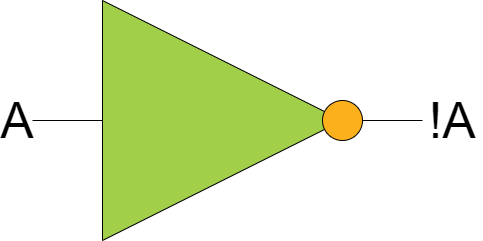
\includegraphics[height=1in]{digital_logic/NOT_gate.png}
        \caption[NOT Gate]{Visual representation of the NOT logical operation with one input and one output.}
    \end{figure}

    \pagelayout{wide} % Remove margins

    \begin{example}[Basic Logic Gates 1] \label{ex:basic-logic-gates-1}
        Let's practice the basic logic gates.
        We will consider a scenario with four inputs and we only want the logical output to be true when inputs A and B and (C or D) are true.
        We can set this up as the expression:
        \begin{equation*}
            (A \cdot B) + (C + D)
        \end{equation*}

        We will then establish the truth table as:
        \begin{center}
            \begin{tabular}{c c c c | c}
                \toprule
                Input D & Input C & Input B & Input A & Output \\
                \midrule
                    0    &    0     &    0     &    0     &    0    \\
                    0    &    0     &    0     &    1     &    0    \\
                    0    &    0     &    1     &    0     &    0    \\
                    0    &    0     &    1     &    1     &    0    \\
                    0    &    1     &    0     &    0     &    0    \\
                    0    &    1     &    0     &    1     &    0    \\
                    0    &    1     &    1     &    0     &    0    \\
                    0    &    1     &    1     &    1     &    1    \\
                    1    &    0     &    0     &    0     &    0    \\
                    1    &    0     &    0     &    1     &    0    \\
                    1    &    0     &    1     &    0     &    0    \\
                    1    &    0     &    1     &    1     &    1    \\
                    1    &    1     &    0     &    0     &    0    \\
                    1    &    1     &    0     &    1     &    0    \\
                    1    &    1     &    1     &    0     &    0    \\
                    1    &    1     &    1     &    1     &    1    \\
                \bottomrule
            \end{tabular}
        \end{center}
        Here, we can easily see that there are 3 input sets that will allow a logical true output in our scenario.

        Next, we can create a visual representation of this scenario:
        \begin{center}
            
\includegraphics[height=2.5in]{digital_logic/BasicGatesEx1.png}
        \end{center}

        While the required input set to get a logical true output is not obvious, it is a little easier to understand the "logic flow" through our scenario and we can test different input ideas and comprehend what is occurring a little easier.

        % \todo{Insert Arduino example!}
    \end{example}

    \begin{example}[Basic Logic Gates 2] \label{ex:basic-logic-gates-2}
        In this scenario, we are going to add a NOT gate and change the output conditions.
        Here we are looking for A and B or not (C or D).
        As before, we set up the scenario as the expression:
        \begin{equation*}
            A \cdot B + \overline{(C + D)}
        \end{equation*}

        We can also build the truth table:
        \begin{center}
            \begin{tabular}{c c c c | c}
                \toprule
                Input D & Input C & Input B & Input A & Output \\
                \midrule
                    0    &    0     &    0     &    0     &    1    \\
                    0    &    0     &    0     &    1     &    1    \\
                    0    &    0     &    1     &    0     &    1    \\
                    0    &    0     &    1     &    1     &    1    \\
                    0    &    1     &    0     &    0     &    0    \\
                    0    &    1     &    0     &    1     &    0    \\
                    0    &    1     &    1     &    0     &    0    \\
                    0    &    1     &    1     &    1     &    1    \\
                    1    &    0     &    0     &    0     &    0    \\
                    1    &    0     &    0     &    1     &    0    \\
                    1    &    0     &    1     &    0     &    0    \\
                    1    &    0     &    1     &    1     &    1    \\
                    1    &    1     &    0     &    0     &    0    \\
                    1    &    1     &    0     &    1     &    0    \\
                    1    &    1     &    1     &    0     &    0    \\
                    1    &    1     &    1     &    1     &    1    \\
                \bottomrule
            \end{tabular}
        \end{center}
        We can see from the table that we have several more conditions that will result in a true output from our expression!

        If we create a diagram of this scenario, we get the following:
        \begin{center}
            
\includegraphics[height=2.5in]{digital_logic/BasicGatesEx2.png}
        \end{center}

        % \todo{Insert Arduino example!}
    \end{example}

    \pagelayout{margin} % Restore margins

    \subsection{Combination Logical Operators}
    As we can see from the previous example, we can combine gates together to change their logical outputs accordingly.
    Adding a NOT gate to the first OR gate gave several more conditions that would make the system output a logical true value.
    However, it can be unnecessarily clumsy to draw a gate immediately followed by a NOT gate, so we can combine them together into a single gate.

    \paragraph*{The NAND operator} is a combination NOT and AND (NOT-AND, NAND) operation. 
    This means the operation outputs a logical true value only when both input 1 \textit{and} input 2 are \textit{not} true.
    \marginnote{For you computer storage afficionados out there, NAND flash memory is one of the predominant architectures for high speed, solid state drives.}
    This can be represented by the expression and truth table below:
    \begin{equation*}
        \overline{(A \cdot B)}
    \end{equation*}

    \begin{table}[h!]
        \labtab{nand_truth_table}
        \begin{tabular}{c c | c}
            \toprule
            $A$ & $B$ & $\overline{(A \cdot B)}$  \\
            \midrule
             0  &  0  &    1    \\
             0  &  1  &    1    \\
             1  &  0  &    1    \\
             1  &  1  &    0    \\
            \bottomrule
        \end{tabular}
    \end{table}

    This gate is graphically represented by the symbol. 
    As you can see, the NAND gate is distinguished from its former identity by the circle at the front of the gate.
    You may also notice that this is the same circle present at the tip of the NOT gate, clearly relating the two.
    \begin{figure}[h!]
        \labfig{nand_gate}
        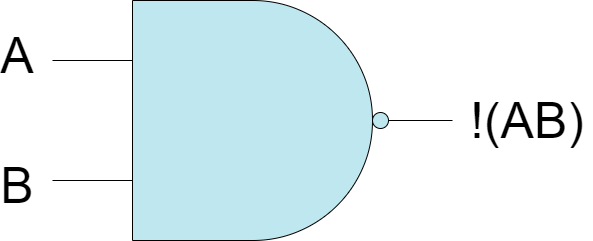
\includegraphics[height=1in]{digital_logic/NAND_gate.png}
        \caption[NAND Gate]{Visual representation of the NAND logical operation with two inputs and one inverted output.}
    \end{figure}

    \paragraph*{The NOR gate} is a combination NOT and OR (NOT-OR, NOR) operation.
    The bottom symbols in Example \ref{ex:basic-logic-gates-2} can be combined into this single operation to achieve the same effect in a more space-efficient manner.
    This gate has a similar equation to its predecessor, looking like:
    \begin{equation*}
        \overline{(A + B)}
    \end{equation*}

    It is represented by the truth table:
    \begin{table}[h!]
        \labtab{nand_truth_table}
        \begin{tabular}{c c | c}
            \toprule
            $A$ & $B$ & $\overline{(A + B)}$  \\
            \midrule
             0  &  0  &    1    \\
             0  &  1  &    0    \\
             1  &  0  &    0    \\
             1  &  1  &    0    \\
            \bottomrule
        \end{tabular}
    \end{table}

    And the graphical representation below. 
    Again, notice how the only distinguishing factor between a NOR and OR gate is the circle at the tip of the gate.
    \begin{figure}[h!]
        \labfig{nor_gate}
        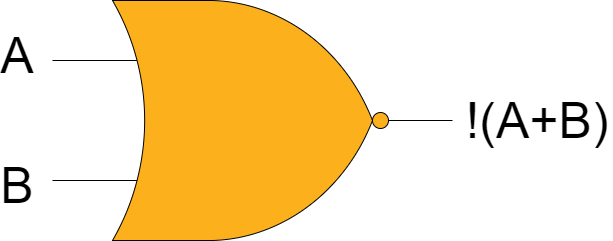
\includegraphics[height=1in]{digital_logic/NOR_gate.png}
        \caption[NOR Gate]{Visual representation of the NOR logical operation with two inputs and one inverted output.}
    \end{figure}

    \subsection{Advanced Logical Operators}
    Sometimes it is desirable to have some more limited conditions in which an operation will output a logical true.
    
    \paragraph*{The exclusive OR operation} can be achieved by combining multiple operations like so:
    \begin{equation*}
        (A+B) \cdot \overline{(A \cdot B)}
    \end{equation*}
    However, this can be a hassle to write, so we can simplify the expression using a special operator symbol $\oplus$.
    This allows us to write an equivalent expression for the exclusive OR operation:
    \begin{equation*}
        A \oplus B
    \end{equation*}

    This operation can also be expressed by the truth table and gate visualization below:
    \begin{table}[h!]
        \labtab{xor_truth_table}
        \begin{tabular}{c c | c}
            \toprule
            $A$ & $B$ & $(A \oplus B)$  \\
            \midrule
             0  &  0  &    0    \\
             0  &  1  &    1    \\
             1  &  0  &    1    \\
             1  &  1  &    0    \\
            \bottomrule
        \end{tabular}
    \end{table}

    As we can see from the truth table, this operation can be best explained as "\textit{either or, but never both}"

    \begin{figure}[h!]
        \labfig{xor_gate}
        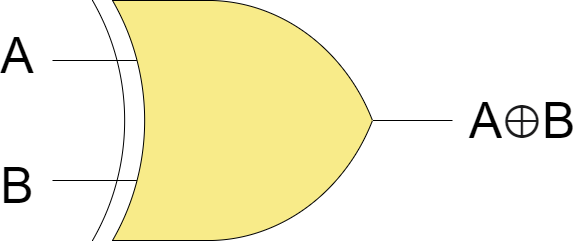
\includegraphics[height=1in]{digital_logic/XOR_gate.png}
        \caption[NOR Gate]{Visual representation of the NOR logical operation with two inputs and one output.}
    \end{figure}

    Note that the visual gate for the exclusive OR is differentiated from its basic counterpart by the additional arc at the back of the gate.

    \paragraph*{The XNOR operation} is just like previous combination operations where we combine the XOR operation with a NOT operation.
    This changes the input requirements for a logical true output to both inputs have to be the same, rather than they have to be different.
    This operation is created by combining multiple operations ike so:
    \begin{equation*}
        \overline{(A+B)} \cdot (A \cdot B)
    \end{equation*}
    And again, these complex combinations can be simplified by adding the $\oplus$ operator an negating it:
    \begin{equation*}
        \overline{(A \oplus B)}
    \end{equation*}

    This results in a truth table and graphical representation shown below:
    \begin{table}[h!]
        \labtab{xnor_truth_table}
        \begin{tabular}{c c | c}
            \toprule
            $A$ & $B$ & $\overline{(A \oplus B)}$  \\
            \midrule
             0  &  0  &    0    \\
             0  &  1  &    1    \\
             1  &  0  &    1    \\
             1  &  1  &    0    \\
            \bottomrule
        \end{tabular}
    \end{table}

    \begin{figure}[h!]
        \labfig{xnor_gate}
        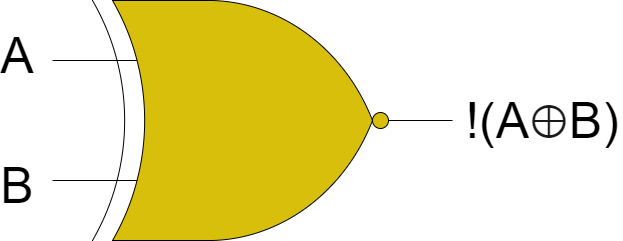
\includegraphics[height=1in]{digital_logic/XNOR_gate.png}
        \caption[XNOR Gate]{Visual representation of the XNOR logical operation with two inputs and one inverted output.}
    \end{figure}

    \pagelayout{wide} % Remove margins

    \begin{example}[Advanced Logic Gates] \label{ex:advanced-logic-gates}
        For this example, we will be combining everything we have learned through this section into a single problem.
        We will start with the logic gate diagram shown below:
        \begin{center}
            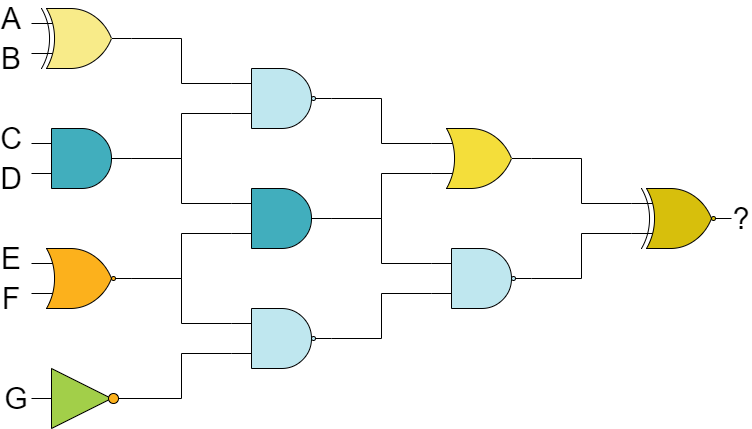
\includegraphics[height=2.5in]{digital_logic/AdvancedGatesEx.png}
        \end{center}

        Let's start by breaking down the first third of the diagram into three regions (I-I, I-II, I-III) and determining their individual logical expressions.
        \begin{center}
            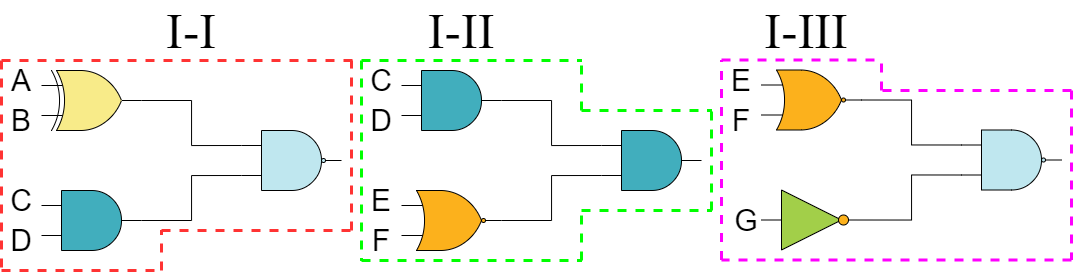
\includegraphics[height=1.5in]{digital_logic/AdvancedGatesEx_I.png}
        \end{center}

        The first section, I-I has an output determined by the expression:
        \begin{equation*}
            \overline{(A \oplus B) \cdot (C \cdot D)}
        \end{equation*}

        The second section, I-II is determined by the expression:
        \begin{equation*}
            \left[ (C \cdot D) \cdot \overline{(E + F)} \right]
        \end{equation*}

        The final section, I-II can be expressed by:
        \begin{equation*}
            \overline{\overline{(E + F)} \cdot \bar{G]}
        \end{equation*}

        Next, let's breakdown the middle of the diagram into two more regions we will denote as II-I and II-II.
        Again, we will determine the logical expression that represents each of these individual sectors.
    \end{example}

    \pagelayout{margin} % Restore margins